\author{Weissengruber Nina}
Die Aufgabenstellungm der vorliegenden Arbeit, ist das Erstellen einer Fragebogen Plattform, 
bei der sichergestellt wird, dass die erhobenen Daten unter der Kontrolle des Fragenstellers bleiben, um so sämtliche datenschutzrechtlichen Aspekte zu erfüllen

In folgender Abbildung sieht man das Use-Case Diagramm für unsere Arbeit.

\begin{figure}[!htb]
    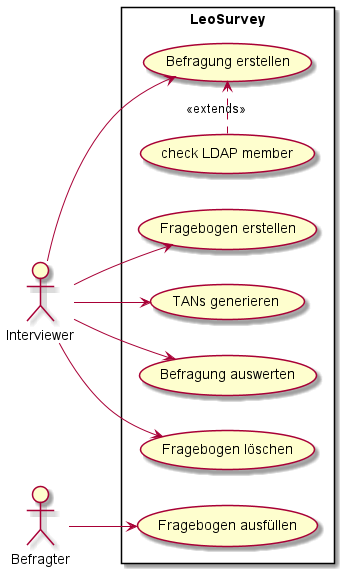
\includegraphics[width=0.5\textwidth]{pics/ucd.png}
    \centering
    \caption{Use Case Diagramm}
\end{figure}

Zunächst ist ein Fragebogen mit seinen Fragen zu erstellen. 
Anschließend wird eine Umfrage geplant (Bezeichnung der Umfrage, ev. Zeitraum der Umfrage, 
Teilnehmer der Umfrage). Danach werden Transaktionscodes (TAN) erstellt, 
um den Befragten eine anonyme Teilnahme an der Umfrage zu ermöglichen. Schließlich werden diese 
TANS an die Befragten übermittelt, woraufhin diese die Fragen des Fragebogens beantworten.
